\let\negmedspace\undefined
\let\negthickspace\undefined
\documentclass[journal]{IEEEtran}
\usepackage[a5paper, margin=10mm, onecolumn]{geometry}
%\usepackage{lmodern} % Ensure lmodern is loaded for pdflatex
\usepackage{tfrupee} % Include tfrupee package

\setlength{\headheight}{1cm} % Set the height of the header box
\setlength{\headsep}{0mm}     % Set the distance between the header box and the top of the text

\usepackage{gvv-book}
\usepackage{gvv}
\usepackage{cite}
\usepackage{amsmath,amssymb,amsfonts,amsthm}
\usepackage{algorithmic}
\usepackage{graphicx}
\usepackage{textcomp}
\usepackage{xcolor}
\usepackage{txfonts}
\usepackage{listings}
\usepackage{enumitem}
\usepackage{mathtools}
\usepackage{gensymb}
\usepackage{comment}
\usepackage[breaklinks=true]{hyperref}
\usepackage{tkz-euclide} 
\usepackage{listings}
% \usepackage{gvv}                                        
\def\inputGnumericTable{}                                 
\usepackage[latin1]{inputenc}                                
\usepackage{color}                                            
\usepackage{array}                                            
\usepackage{longtable}                                       
\usepackage{calc}                                             
\usepackage{multirow}                                         
\usepackage{hhline}                                           
\usepackage{ifthen}                                           
\usepackage{lscape}
\begin{document}

\bibliographystyle{IEEEtran}
\vspace{3cm}




\title{
%	\logo{
17-03-2021 Shift-1

\large{EE1030 : Matrix Theory}

Indian Institute of Technology Hyderabad
%	}
}
\author{Satyanarayana Gajjarapu

AI24BTECH11009
}	





\maketitle




\bigskip

\renewcommand{\thefigure}{\theenumi}
\renewcommand{\thetable}{\theenumi}


\section{\large Shift-1(16-30)}


\begin{enumerate}
\item Two dice are rolled. If both dices have six faces numbered 1, 2, 3, 5, 7 and 11, then the probability that the sum of the numbers on the top faces is less than or equal to 8 is:
\begin{enumerate}
    \item $\frac{17}{36}$
    \item $\frac{4}{9}$
    \item $\frac{5}{12}$
    \item $\frac{1}{2}$\\
\end{enumerate}
\item The inverse of $y = 5^{\log{x}}$ is:
  \begin{enumerate}
      \item $x = 5^{\log{y}}$
      \item $x = y^{\log{5}}$
      \item $x = y^{\frac{1}{\log{5}}}$
      \item $x = 5^{\frac{1}{\log{y}}}$\\
  \end{enumerate}
\item In a school, there are three types of games to be played. Some of the students play two types of games, but none play all three games. Which Venn diagrams can justify the above statements.
\begin{figure}[h!]
	    \centering
	    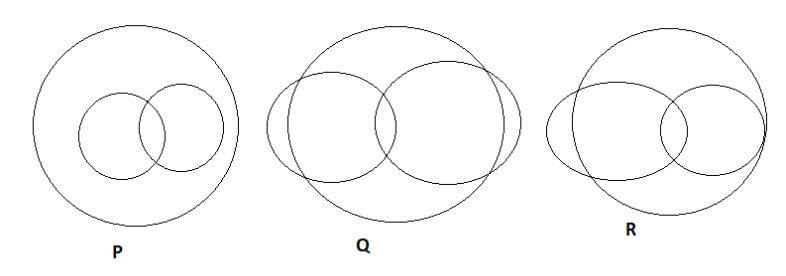
\includegraphics[width=0.7\linewidth]{figs/Q3.png}
     \begin{enumerate}
         \item P and R
         \item P and Q
         \item None of these
         \item Q and R\\
     \end{enumerate}
    \end{figure}
 \item The area of the triangle with vertices $A (z)$, $B (iz)$ and $C (z + iz)$ is:
 \begin{enumerate}
     \item $\frac{1}{2}\abs{z+iz}^2$
     \item 1
     \item $\frac{1}{2}$
     \item $\frac{1}{2}\abs{z}^2$\\
 \end{enumerate}
\item The value of $\lim_{x\rightarrow 0+} \frac{\sbrak{\cos^{-1}\brak{x - \sbrak{x}^2}\cdot\sin^{-1}\brak{x - \sbrak{x}^2}}}{\sbrak{x - x^3}}$, where \sbrak{x} denote the greatest integer $\leq x$ is:
\begin{enumerate}
    \item 0
    \item $\frac{\pi}{4}$
    \item $\frac{\pi}{2}$
    \item $\pi$\\
\end{enumerate}
\item  Let there be three independent events $E_1$, $E_2$ and $E_3$. The probability that only $E_1$ occurs is $\alpha$, only $E_2$ occurs is $\beta$ and only $E_3$ occurs is $\gamma$. Let $'p'$ denote the probability of none of the events that occur that satisfies the equations $\brak{\alpha - 2\beta}p = \alpha\beta$ and $\brak{\beta - 3\gamma}p = 2\beta\gamma$. All the given probabilities are assumed to lie in the interval \brak{0, 1}. Then, $\frac{\sbrak{\text{probability of occurrence of} E_1}}{\sbrak{\text{probability of occurrence of} E_3}}$ is equal to \_\_\_\_\_\_  \\
\item If the equation of the plane passing through the line of intersection of the planes $2x - 7y + 4z - 3 = 0$, $3x - 5y + 4z + 11 = 0$ and the point \brak{-2, 1, 3} is $ax + by + cz - 7 = 0$, then the value of $2a + b + c - 7$ is \_\_\_\_\_\_ \\
\item If $A$=\sbrak{\begin{matrix}
     2 & 3 \\ 0 & -1
 \end{matrix}}, then the value of $\det{\brak{A^4}} + \det{\brak{A^{10} - adj\brak{2A}^{10}}}$ is equal to \_\_\_\_\_\_ \\
\item The minimum distance between any two points $P_1$ and $P_2$ while considering point $P_1$ on one circle and point $P_2$ one the other circle for the given circles' equations $x^2 + y^2 - 10x - 10y + 41 = 0$ and $x^2 + y^2 - 24x - 10y + 160 = 0$ \_\_\_\_\_\_ \\
\item If $\brak{2021}^{3762}$ is divided by 17, then the remainder is \_\_\_\_\_\_ \\
\item If \sbrak{\cdot} represents the greatest integer function, then the value of $\abs{\int_{0}^{\frac{\sqrt\pi}{2}}\sbrak{\sbrak{x^2} - \cos{x}}dx}$ is \_\_\_\_\_\_ \\
\item If $f\brak{x} = \sin\sbrak{\cos^{-1}\frac{\brak{1-2^{2x}}}{\brak{1+2^{2x}}}}$ and its first derivative with respect to $x$ is $-\frac{b}{a}\log_{e}{2}$ when $x$ = 1, where $a$ and $b$ are integers, then the minimum value of $\abs{a^2 - b^2}$ is \_\_\_\_\_\_ \\
\item If the function $f\brak{x} = \frac{\sbrak{\cos{\brak{\sin{x}}} - \cos{x}}}{x^4}$ is continuous at each point in its domain and $f\brak{0} = \frac{1}{k}$, then $k$ is \_\_\_\_\_\_ \\
\item The maximum value of $z$ in the following equation $z = 6xy + y^2$, where $3x + 4y \leq 100$ and $4x + 3y \leq 75$ for $x \geq$ 0 and $y \geq$ 0 is \_\_\_\_\_\_ \\
\item If $\vec{a} = \alpha i + \beta j + 3k$, $\vec{b} = -\beta i - \alpha j - k$ and $\vec{c} = i -2j - k$, such that $\vec{a}\cdot\vec{b} = 1$ and $\vec{b}\cdot\vec{c} = -3$, then $\frac{1}{3}\brak{\brak{\vec{a}\times\vec{b}}\cdot\vec{c}}$ is equal to \_\_\_\_\_\_ \\
\end{enumerate}
\end{document}

